\renewcommand{\chaptername}{Capitulo}
\chapter{Planteamiento del problema de investigación} 

\section{Introducción}

Hoy día, existen diversos tratados y convenciones internacionales que promueven el Acceso Abierto (AA) del público en general a la literatura científica y académica de manera digital, ya sean revistas científicas o de divulgación, tesis, artículos, memorias de eventos, libros, entre otros, todo de manera gratuita. Esta propuesta fue planteada en la Iniciativa de Budapest \cite{para2010abierto} en 2002, durante un evento organizado por la \textit{Open Society Institute}. Al siguiente año, en 2003, se llevó a cabo la Declaración de Berlín sobre el AA al conocimiento en las ciencias y las humanidades.\newline

El AA (en inglés \textit{Open Access}) ofrece ventajas tales como \textit{incremento en la difusión e impacto} de la producción científica de Instituciones de Edu\-cación superior (IES) y Centros de Investigación (CI); \textit{rendición de cuentas transparente} ante la sociedad con respecto a la inversión pública; \textit{fomento de la producción} científica y académica incrementando las posibilidades de acceso por parte de los usuarios finales; \textit{dis\-mi\-nu\-ción en la brecha} de acceso a la información entre IES, CI, comunidades locales, nacionales e internacionales; \textit{garantiza la preservación electrónica} de los recursos documentales \cite{BeneficiosAA}. Entre los beneficiarios del AA están los autores, las comunidades científicas y académicas, así como los usuarios finales.\newline

El paradigma del AA se relaciona con el desarrollo e implementación de repo\-sitorios digitales cuyo propósito es ser un medio de divulgación (\textit{ruta verde}) o de publicación a través de revistas científicas (\textit{ruta dorada}), de los contenidos producidos por una institución o comunidad.\newline

\subsection{Panorama general de los repositorios digitales}

Al mes de Diciembre de 2018, según el sitio OpenDOAR \cite{OpenDOAR}, directorio de repositorios de AA de la Universidad Nottingham, existían tres mil setecientos setenta y nueve repositorios de AA alrededor del mundo, de los cuales poco menos de la mitad se encuentran en Europa (46\%), el 27\% en Norteamérica y sólo el 0.9\% en México. En nuestro país, el Repositorio Nacional \cite{RepositorioNacional} reporta la existencia de 44 repositorios de Ciencia Abierta (CA) e INDEXE \cite{RI_REMERI} contabiliza noventa y ocho repositorios institucionales (RIs), los cuales están comprometidos con la divulgación de sus contenidos institucionales y temáticos bajo las políticas de AA.\newline

En cuanto al tipo de \textit{software} empleado para la implementación de repositorios digitales (RDs), OpenDOAR \cite{OpenDOAR} señala que las cuatro plataformas más empleadas en el mundo son: \textit{DSpace} \cite{DSpaceRef} (44.2\%), \textit{EPrints} (13.4\%), \textit{Digital Commons} (4.7\%) y \textit{WEKO} (2.7\%). A diferencia de \textit{Digital Commons} que es un \textit{software} licenciado por la empresa \textit{Beprees}, \textit{DSpace} y \textit{EPrints} cuentan con licencia libre, por lo que su uso se ha extendido en múltiples IES, CI y otros.\newline

\textit{DSpace} \cite{DSpaceRef} es un proyecto que fue desarrollado en sus inicios por el Instituto Tecnológico de Massachusetts - MIT en el año 2002 en conjunto con los Laboratorios HP. Actualmente, es lidereado por la fundación \textit{DuraSpace} que entre sus objetivos se encuentran la innovación en tecnologías de AA y basadas en nube, principalmente para bibliotecas, universidades, CIs y organizaciones de patrimonio cultural, brindando soporte para RIs, almacenamiento de tesis electrónicas, administración de registros electrónicos, preservación digital y publicación.\newline

\textit{EPrints} \cite{EPrints} es un software de uso libre desarrollado en el año 2000 por la Universidad de Southampton, UK, esta plataforma brinda soporte libre para la preservación, diseminación y generación de reportes para instituciones que requieran que servicios de AA, también permite el desarrollo de repositorios de educación abierta (en inglés \textit{Open Education}) y bancos de datos para investigación (en inglés \textit{Research Data}). Eprints ofrece además integración robusta con las redes sociales, por lo que muchas instituciones lo emplean como medio de integración entre sus comunidades estudiantiles y académicas.\newline

Existen otras alternativas de software para la implementación de RDs tales como VIVO \cite{VivoWeb}, que es una plataforma de acceso abierto desarrollada por la Universidad de Cornell, en el año 2003, que incluye un módulo de ontologías como \textit{Dublin Core} \footnote{Disponible en http://dublincore.org/} , \textit{Bibliographic Ontology} \footnote{Disponible en http://bibliontology.com/}, \textit{FOAF} \footnote{Disponible en http://www.foaf-project.org/} y \textit{SKOS} \footnote{Disponible en http://www.w3.org/2004/02/skos/}. Por otro lado, Virtuoso es una plataforma desarrollada en España por la empresa OpenLink \cite{VirtuosoRef}; algunas de sus aplicaciones son servicios web simples, bases de datos, web semántica, sistemas inteligentes, exportación e importación de documentos en múltiples formatos, documentos compartidos a través de la nube, blogs, wikis, correo personalizado y modelos de negocios.\newline

\subsection{Tecnologías semánticas en los repositorios}

Como se ha descrito anteriormente, existen RIs actualmente implementados en di\-fe\-ren\-tes IES o CIs, sin embargo, éstos no cuentan con las tecnologías semánticas implementadas de manera inicial, por lo que se presentan diferentes inconvenientes tales como:

\begin{itemize}
\item \textit{Inconsistencia} de los datos cuando al menos dos propiedades definidas dentro del diseño de la base de datos no relacional u ontología se contraponen entre sí.
\item \textit{Ambigüedad} en la interpretación de los datos, es decir, que el resultado de alguna consulta o búsqueda arroja información que cuyo significado no es congruente con lo que el usuario pretende encontrar.
\item \textit{Errores de definición} en el dominio de una ontología, lo cual repercute en la delimitación del rango.
\item \textit{Problemas} para la integración de una base de conocimiento útil.
\end{itemize}

Así pues, las tecnologías semánticas estan soportadas en una modelo representacional de los datos llamadas ontologías --- abundar mas en las ontologías???.

Entre las ventajas que representa el uso de las ontologías y los modelos de datos no relacionales se mencionan las siguientes: \cite{ASWebQuest} \cite{GuideCreatingOntology}

\begin{itemize}
\item \textit{Intercambio de información} entre aplicaciones, programas y/o plataformas través del uso del lenguaje XML.
\item \textit{Datos incompletos}, es decir, a pesar de que algunos datos no estén contenidos en la base, aún así la ontología puede arrojar resultados a las consultas formuladas por los usuarios.
\item \textit Las ontologías permiten el manejo de mayor {tipos de datos} que en una base de tipo relacional, lo cual permite realizar consultas específicas.
\item \textit Permiten la {reutilización del conocimiento}, es decir, al recopilar la información, ésta se encuentra a disposición de los usuarios para consultar o acrecentar la información existente.
\item \textit{Analizar el dominio }del conocimiento, fijando límites entre éste y el conocimiento operacional.

\end{itemize}

Por lo anterior expuesto, se propone el siguiente objetivo general y un conjunto de tareas individuales como parte de objetivos particulares que permitan alcanzar el cumplimiento general del proyecto que se plantea.

\section{Objetivos}
\subsection{Objetivo general}
Analizar la representación y recuperación de información semántica 
en repositorios que implementan políticas de acceso abierto para implementar un servicio web RN-REST de búsqueda semántica a los datos del RI-UPPUe.
\subsection{Objetivos especificos}
\begin{itemize}
     \item  Ampliar el modelado del RI-UPPue representado en la versión 1.0 de la ontología Onto4UPPue extendiendo su expresividad.

     \item Analizar la funcionalidad del componente RDF de la plataforma DSpace 6.2, Virtuoso y Vivo relacionada con la representación y recuperación de información semántica.
     
     \item Implementar un servicio web de recuperación de información semántica que agregue valor a datos provenientes de al menos dos RIs que implementen el protocolo de interoperabilidad OAI-PMH \footnote{Open Archives Initiative – Protocol for Metadata Harvesting}.
   \end{itemize}
   
\subsection{Tareas}

Para el desarrollo del servicio web se plantean tareas que ayudan a cumplir con los tres objetivos específicos, las cuales se describen en la figura \ref{actividades_objetivos} .\newline

\begin{figure}[!ht]
    \centering
    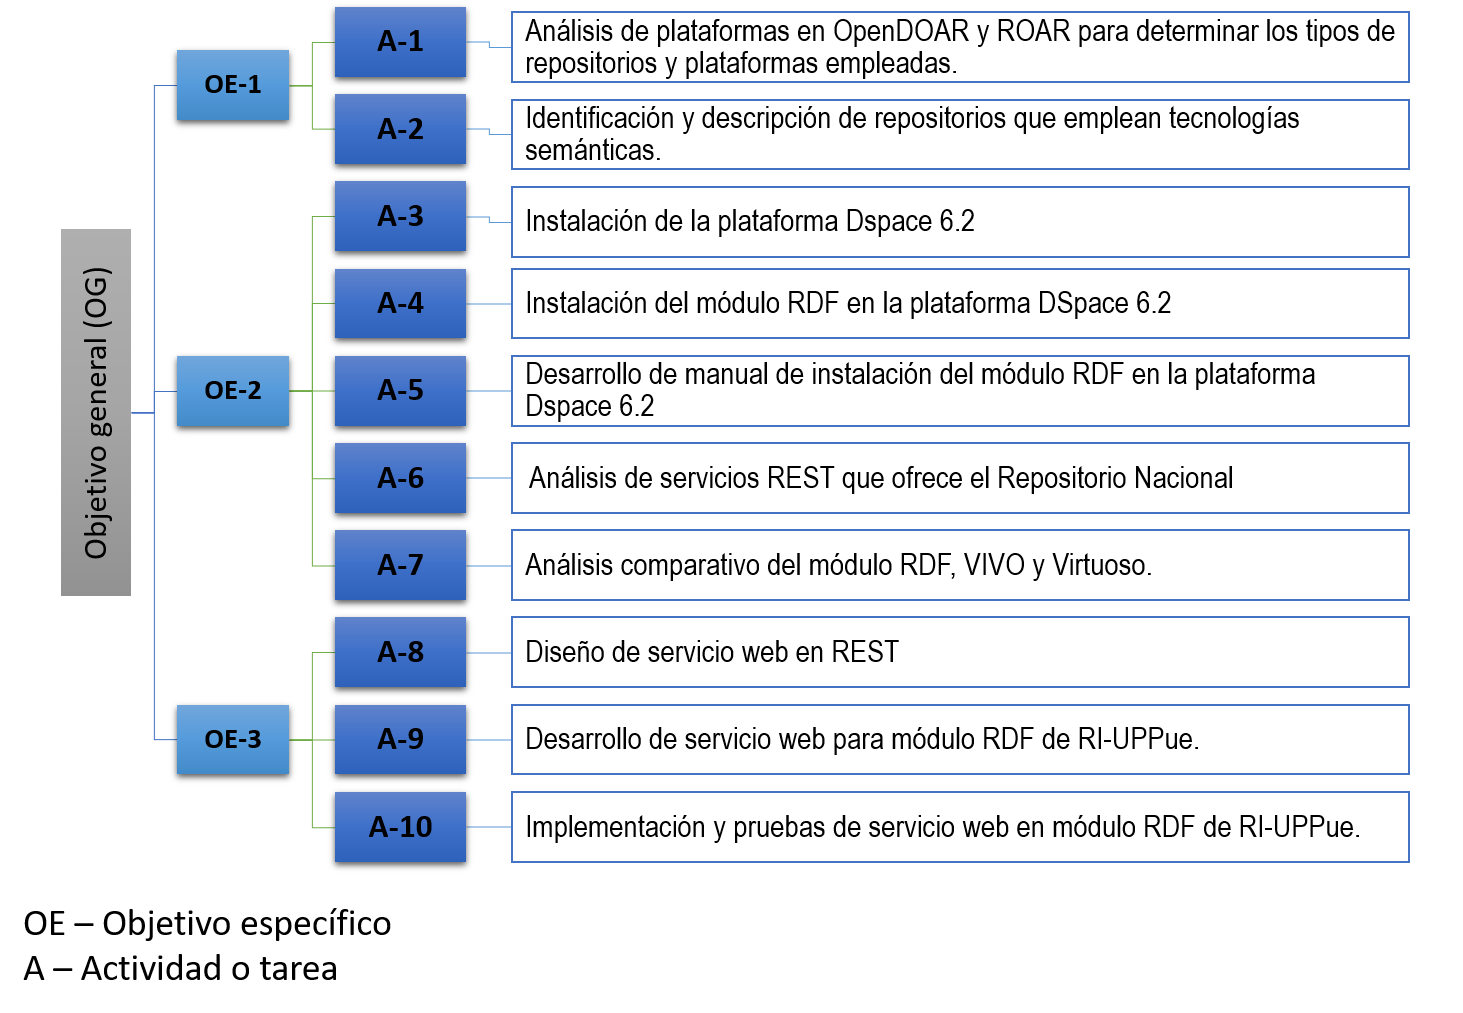
\includegraphics[width=12cm]{figures/Actividades_Dic_2018.png} %NOMBRE DE LA FIGURA y TAMAÑO
    \caption{Tareas a desempeñar para el desarrollo del servicio web} %PIE DE LA IMAGEN
    \label{actividades_objetivos}
\end{figure}

\section{Justificación}

En los últimos años, diferentes IES, CIs y comunidades se han sumado el esfuerzo de promover el AA a sus contenidos científicos, aprovechando al mismo tiempo los beneficios generados por la implantación de un RD.\newline

En México, más del 45\% de RI's pertenecen a instituciones públicas \cite{RI_REMERI}, siendo la Universidad Nacional Autónoma de México - \textit{UNAM} la institución con mayor número de repositorios y documentos publicados. En este sentido, la Universidad Politécnica de Puebla actualmente participa en un proyecto que implementa un Repositorio Institucional (\textit{RI-UPPuebla}) en el cual sus investigadores, alumnos de posgrado y comunidad universitaria en general, difundirá y preservará contenidos de carácter científico y académico en AA, donde los beneficios esperados por tipo de usuario serán:

- A los investigadores: 
	\begin{itemize}
	\item \textit{Publicación de los resultados} de su investigación al interior y exterior de la comunidad universitaria.
    \item \textit{Mayor número de citas}, al ser más accesible al público, causando mayor impacto.
    \item \textit{Gestión} de los derechos de autor.
    \item \textit{Acceso permanente} a las publicaciones ya que los accesos no se modifican, como suele ocurrir en otros medios digitales.
    \item \textit{Almacenamiento flexible}, al permitir almacenar cualquier tipo de documentos como artículos, tesis, revistas, memorias, videos, audios, etc. en formatos digitales.
	\end{itemize}
	
- A la UPPue:
	\begin{itemize}
	\item \textit{Recopilación y divulgación} la producción científica y académica de la institución.
    \item \textit{Visibilidad e impacto}, ya que al colocar mayor número de publicaciones en las búsquedas de diversos motores, posicionará a la UPPue como referente en citas de docentes y estudiantes.
    \item \textit{Banco de conocimientos hacia el futuro}, al preservar las obras, el acervo do\-cu\-mental y de conocimientos crecerá con el paso del tiempo, lo cual fomentará mayor actividad de investigación entre la comunidad universitaria, al contar con las bases científicas realizadas por sus pares e incluso sus predecesores.
	\end{itemize}
	
- A la comunidad universitaria:
  \begin{itemize}
  \item \textit{Acceso libre y gratuito} a obras científicas y académicas serias y de origen confiable.
  \item \textit{Cooperación y acceso} compartido entre las IES que conforman comunidades de conocimiento de la región, del país o de la comunidad internacional.
  \item \textit{Evidencias} tangibles de los resultados generados a través de la inversión pública o privada de recursos en el campo de la investigación científica o académica.
  \end{itemize}

Además, como parte del proceso de consolidación del RI-UPPue, es necesario identificar áreas de oportunidad que permitan brindar una experiencia más satisfactoria para los usuarios finales (público en general), es decir, es indispensable ofrecer de igual manera, un canal o medio que posibilite el acceso de manera sencilla a la información requerida, teniendo la posibilidad de establecer cuestionamientos y obteniendo respuestas claras y concisas a estos con base en la aplicación de tecnologías semánticas.\newline

Si bien la mayoría de las IES, CI u otro tipo de organizaciones implementan herra\-mi\-en\-tas para la concentración y administración de su información dentro de bases de datos, es necesario la integración de tecnologías semánticas para transformar los datos en conocimiento, lo cual permite acceder a la información desde un punto de vista conceptual y no textual.\newline

En suma, el desarrollo e implantación de un módulo de consultas semánticas para los usuarios finales, permitirá extender los mecanismos de búsqueda y recuperación relacionada con los recursos; en comparación con los mecanismos provistos en el RI-UPPue, los usuarios pueden tener una mejor experiencia en la búsqueda de información, ya que éstos métodos de consulta reducen la ambigüedad con el objeto de brindar resultados precisos de acuerdo a las necesidades de los usuarios finales.\newline


